\section{MOPEX-2 (model ID: 30)}
The MOPEX-2 model (fig.~\ref{fig:30_schematic}) is part of a model improvement study that investigates the relationship between dominant processes and model structures for 197 catchments in the MOPEX database \citep{Ye2012}. It has 5 stores and 7 parameters ($T_{crit}$, $ddf$, $S_{b1}$, $t_w$, $t_u$, $S_e$ and $t_c$). The model aims to represent:

\begin{itemizecompact}
\item Snow accumulation and melt;
\item Saturation excess flow;
\item Infiltration to deeper soil layers;
\item A split between fast and slow runoff.
\end{itemizecompact}

\subsection{MARRMoT model name}
m\_30\_mopex2\_7p\_5s \\

% Equations
\subsection{Model equations}

% Model layout figure
{ 																	% This ensures it doesn't warp text further down
\begin{wrapfigure}{l}{6cm}
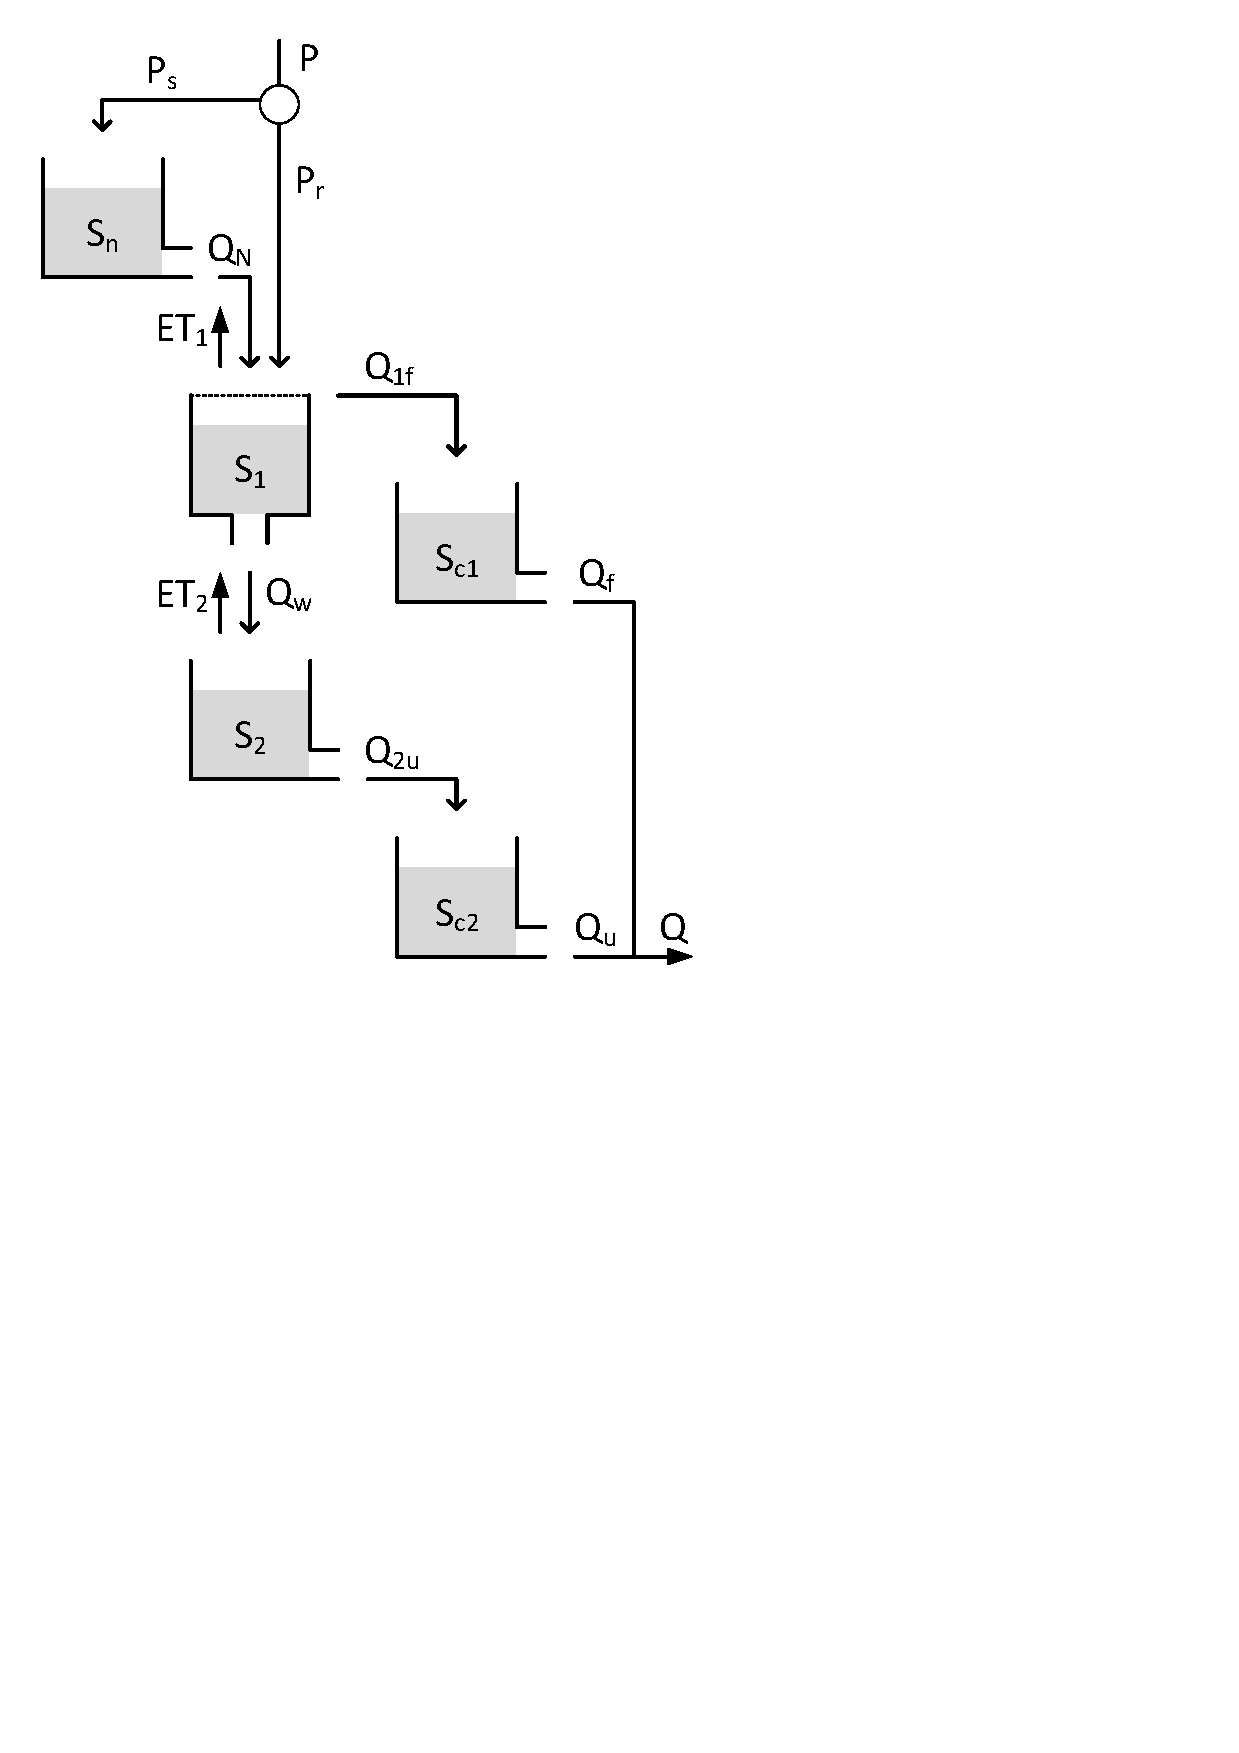
\includegraphics[trim=1cm 13cm 7cm 1cm,width=7cm,keepaspectratio]{./AppA_files/30_schematic.pdf}
\caption{Structure of the MOPEX-2 model} \label{fig:30_schematic}
\end{wrapfigure}

\begin{align}
	\frac{dS_n}{dt} &= P_s-Q_{n} \\
	P_s &= \begin{cases}
		P, &\text{if } T \leq T_{crit} \\
		0, & \text{otherwise} \\
	\end{cases} \\
	Q_n &=\begin{cases}
		ddf*(T-T_{crit}), &\text{if } T > T_{crit} \\
		0, & \text{otherwise} \\
	\end{cases}
\end{align}

Where $S_n$ [mm] is the current snow pack. Precipitation occurs as snowfall $P_s$ $[mm/d]$ when current temperature T $[^oC]$ is below threshold $T_{crit}$ $[^oC]$. Snowmelt $Q_N$ $[mm/d]$ occurs when the temperature rises above the threshold temperature and relies in the degree-day factor $dd$ $[mm/^oC/d]$.

\begin{align}
	\frac{dS_1}{dt} &= P_r-ET_1-Q_{1f}-Q_w \\
	P_r &= \begin{cases}
		P, &\text{if } T > T_{crit} \\
		0, & \text{otherwise} \\
	\end{cases} \\
	ET_1 &= \frac{S_1}{S_{b1}}*Ep\\
	Q_{1f} &= \begin{cases}
		P, &\text{if } S_1 \geq S_{b1} \\
		0, & \text{otherwise} \\
	\end{cases} \\
	Q_w &= t_w*S_1
\end{align}

} % end of wrapfigure fix

Where $S_1$ [mm] is the current storage in soil moisture and $P_r$ precipitation as rain $[mm/d]$. Evaporation $ET_1$ $[mm/d]$ depends linearly on current soil moisture, maximum soil moisture $S_{b1}$ [mm] and potential evapotranspiration $E_p$ [mm/d]. Saturation excess flow $Q_{1f}$  $[mm/d]$ occurs when the soil moisture bucket exceeds its maximum capacity. Infiltration to deeper groundwater $Q_w$  $[mm/d]$ depends on current soil moisture and time parameter $t_w$  $[d^{-1}]$.

\begin{align}
	\frac{dS_2}{dt} &= Q_w-ET_2-Q_{2u}\\
	ET_2 &= \frac{S_2}{S_{e}}*Ep\\
	Q_{2u} &= t_u*S_2
\end{align}

Where $S_2$ [mm] is the current groundwater storage, refilled by infiltration from $S_1$. Evaporation $ET_2$ $[mm/d]$ depends linearly on current groundwater and root zone storage capacity $S_e$ [mm]. Leakage to the slow runoff store $Q_{2u}$ $[mm/d]$ depends on current groundwater level and time parameter $t_u$ $[d^{-1}]$. 

\begin{align}
	\frac{dS_{c1}}{dt} &= Q_{1f}-Q_{f}\\
	Q_f &= t_c*S_{c1}
\end{align}

Where $S_{c1}$ [mm] is current storage in the fast flow routing reservoir, refilled by $Q_{1f}$. Routed flow $Q_f$ depends on the mean residence time parameter $t_c$ $[d^{-1}]$.

\begin{align}
	\frac{dS_{c2}}{dt} &= Q_{2u}-Q_{u}\\
	Q_u &= t_c*S_{c2}
\end{align}

Where $S_{c2}$ [mm] is current storage in the slow flow routing reservoir, refilled by $Q_{2u}$. Routed flow $Q_u$ depends on the mean residence time parameter $t_c$ $[d^{-1}]$. Total simulated flow $Q_t$ $[mm/d]$:

\begin{align}
	Q_t &= Q_f + Q_u
\end{align}

\subsection{Parameter overview}
% Table generated by Excel2LaTeX from sheet 'Sheet1'
\begin{table}[htbp]
  \centering
    \begin{tabular}{lll}
    \toprule
    Parameter & Unit  & Description \\
    \midrule
    $T_{crit}$ & $^oC$ & Threshold temperature for snowfall and melt \\
    $ddf$ & $mm~^oC^{-1}~d^{-1}$ & Degree-day factor \\
    $S_{b1}$ & $mm$  & Maximum soil moisture storage \\
    $t_w$ & $d^{-1}$ & Runoff coefficient \\
    $t_u$ & $d^{-1}$ & Runoff coefficient \\
    $S_e$ & $mm$  & Maximum groundwater storage capacity \\
    $t_c$ & $d^{-1}$ & Runoff coefficient \\
    \bottomrule
    \end{tabular}%
  \label{tab:addlabel}%
\end{table}%

